\documentclass{article}
\usepackage{hyperref}


\usepackage{Sweave}
\begin{document}
\Sconcordance{concordance:hw1_joe_brew_R.tex:hw1_joe_brew_R.Rnw:%
1 4 1 1 0 2 1 1 43 16 1 1 14 1 4 3 1 1 8 1 2 3 1 1 8 7 0 1 1 1 6 3 0 1 %
6 4 0 1 6 4 0 1 6 3 0 1 1 1 7 5 0 1 5 3 0 1 1 1 5 3 0 1 6 4 0 1 6 3 0 1 %
1 1 5 3 0 1 6 10 0 1 5 1 1}


\begin{center}
\huge{HW 1: R supplement}\\
\large{Joe Brew}
\end{center}

\fbox{
  \parbox{\textwidth}{
    \noindent \textbf{Note to professor: } As someone who does most of my work in R, and as an advocate for open-source software, I'll be trying to replicate all assignments and activities from this course in R this semester.  I'm not requesting, nor do I expect, any "credit" for this.  But given that you are also an R user, I'm turning this in (along with the required assignment in ArcGIS) so that you may offer your thoughts or criticism, if you so choose.  }
}\\

\noindent  \\

\noindent What follows is the output of the homework assignment (the two maps), followed by the code used to generate them.  Full code (including the code for this \LaTeX document) is available \href{https://github.com/joebrew/uf/phc6194/hw1}{HERE}.

\newpage
\section*{Question 1}
\begin{center}
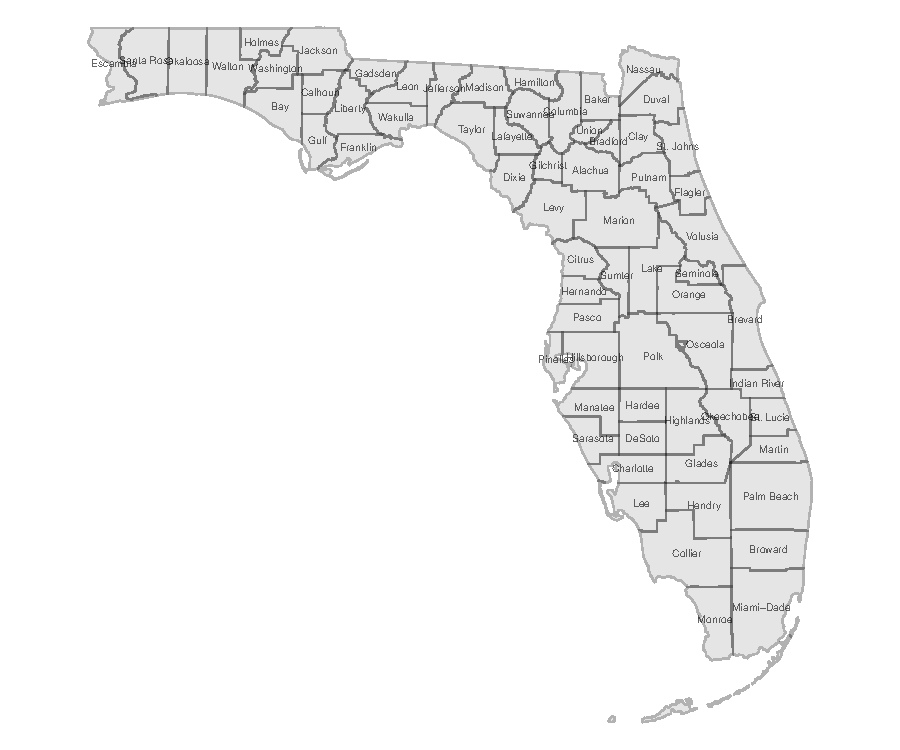
\includegraphics{hw1_joe_brew_R-002}
\end{center}

\section*{Question 2}
\begin{center}
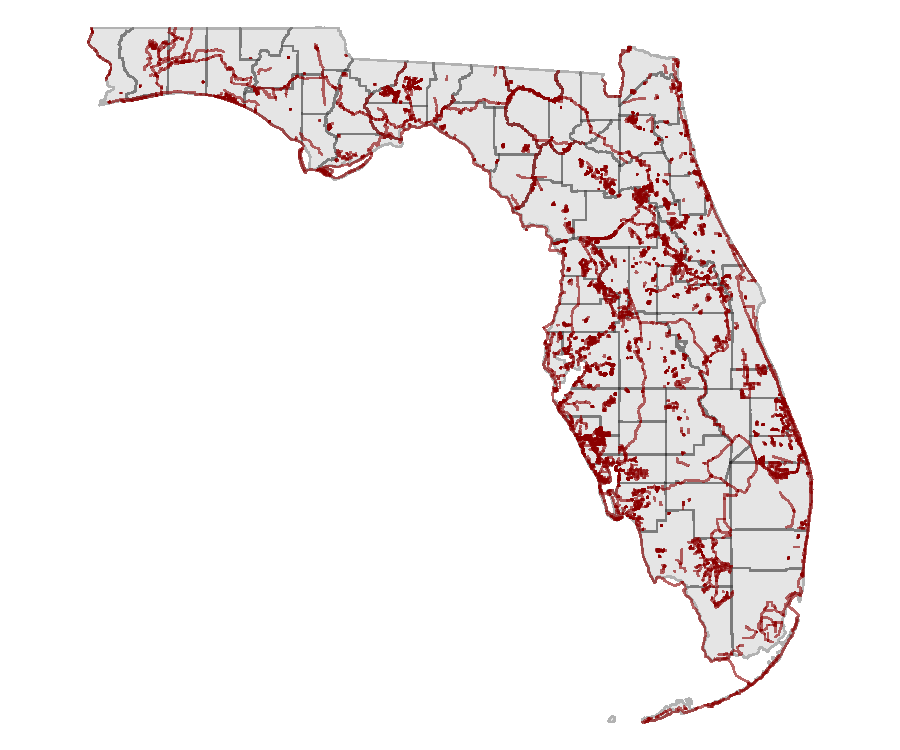
\includegraphics{hw1_joe_brew_R-003}
\end{center}

\newpage
\section*{R Code}
\begin{Schunk}
\begin{Sinput}
> ####################
> # LOAD PACKAGES FOR MAPPING
> ####################
> 
> # IF NOT YET INSTALLED ON YOUR SYSTEM, RUN
> # install.packages("packagename") FIRST
> library(maptools)
> library(rgdal)
> ####################
> # SET WD TO THE HW1 FOLDER
> ####################
> setwd("C:/Users/BrewJR/Documents/uf/phc6194/hw1")
> ####################
> # READ IN FLORIDA COUNTIES SHAPEFILE
> ####################
> fcty2 <- readOGR("FCTY2", 
+                  layer="FCTY2")
> ####################
> # READ IN TRAILS SHAPEFILE
> ####################
> trails <- readOGR("existing_trails_apr09", 
+                  layer="existing_trails_apr09")
> ############
> # EXAMINE PROJECTIONS
> ############
> proj4string(trails)
> proj4string(fcty2)
> #############
> # GIVEN THAT THEY'RE ON DIFFERENT PROJECTION SYSTEMS,
> # PUT TRAILS INTO SAME PROJECTION SYSTEM AS fcty2
> # IN OTHER WORDS, MAKE EVERYTHING LAT LONG
> #############
> trails_latlon <- spTransform(trails, CRS("+init=epsg:4326"))
> ############
> # QUESTION 1 MAP
> ############
> par(mar = rep(0,4))
> par(oma = rep(0,4))
> # PLOT MAP
> plot(fcty2, 
+      border = adjustcolor("black", alpha.f=0.3), 
+      col = adjustcolor("black", alpha.f=0.1))
> # ADD LABELS
> text(coordinates(fcty2),
+      labels = as.character(fcty2$NAME),
+      cex = 0.4,
+      col = adjustcolor("black", alpha.f=0.6))
> ############
> # QUESTION 2 MAP
> ############
> par(mar = rep(0,4))
> par(oma = rep(0,4))
> # PLOT MAP
> plot(fcty2, 
+      border = adjustcolor("black", alpha.f=0.3), 
+      col = adjustcolor("black", alpha.f=0.1))
> # ADD LABELS
> text(coordinates(fcty2),
+      labels = as.character(fcty2$NAME),
+      cex = 0.4,
+      col = adjustcolor("black", alpha.f=0.6))
> 
> 
> 
\end{Sinput}
\end{Schunk}

\end{document}
